\newpage 
\section{Remote Procedure Call (RPC)}

This section will cover the concept of Remote Procedure Calls (RPCs) and how they are used in distributed systems. We will discuss the basic idea of RPCs, how they work, and the challenges they face.
We'll be using the GO RPC library to demonstrate their use with examples.


\begin{Def}[client-server model]

    The client-server model is a distributed application structure that partitions tasks or workloads between the providers of a
     resource or service, \textbf{called servers}, and service requesters, \textbf{called clients}. 
     
     Often clients and servers communicate over a computer network on separate hardware, but both client and server may reside in the same system.

\end{Def}

\begin{Def}[Remote Procedure Call (RPC)]

    A Remote Procedure Call (RPC) is a protocol that allows a \textbf{client} computer request the execution of functions on a separate \textbf{server} computer.

    RPC's abstract the network communication between the client and server enabling developers to write programs that may run on different machines, but appear to run locally.
\end{Def}

\noindent
Now to define the components of an RPC call:
\begin{Def}[RPC Call Stack]

    The RPC call stack facilitates communication between two systems via four layers:
    
    \begin{enumerate}
        \item \textbf{Application Layer:} The highest layer where the client application initiates a function call. On the server side, this layer corresponds to the service handling the request.
        
        \item \textbf{Stub:} A client-side stub acts as a proxy for the remote function, \textbf{marshaling arguments} (converting them into a transmittable format) and forwarding them to the RPC library. On the server side,
        a corresponding stub, \textbf{the dispatcher}, receives the request, unmarshals the data, and passes it to the actual function.
        
        \item \textbf{RPC Library:} The RPC runtime that manages communication between the client and server, ensuring request formatting, serialization, and deserialization.
        
        \item \textbf{OS \& Networking Layer:} The lowest layer, responsible for transmitting RPC request and response messages over the network using underlying transport protocols.
    \end{enumerate}
    
    The request message travels from the client's application layer down through the stack and across the network to the server. The server processes the request in reverse, executing the function and returning the result to the client.
\end{Def}
    
\newpage 

\noindent
To illustrate the RPC call stack, observe the following diagram:
\begin{figure}[h]
    \centering
    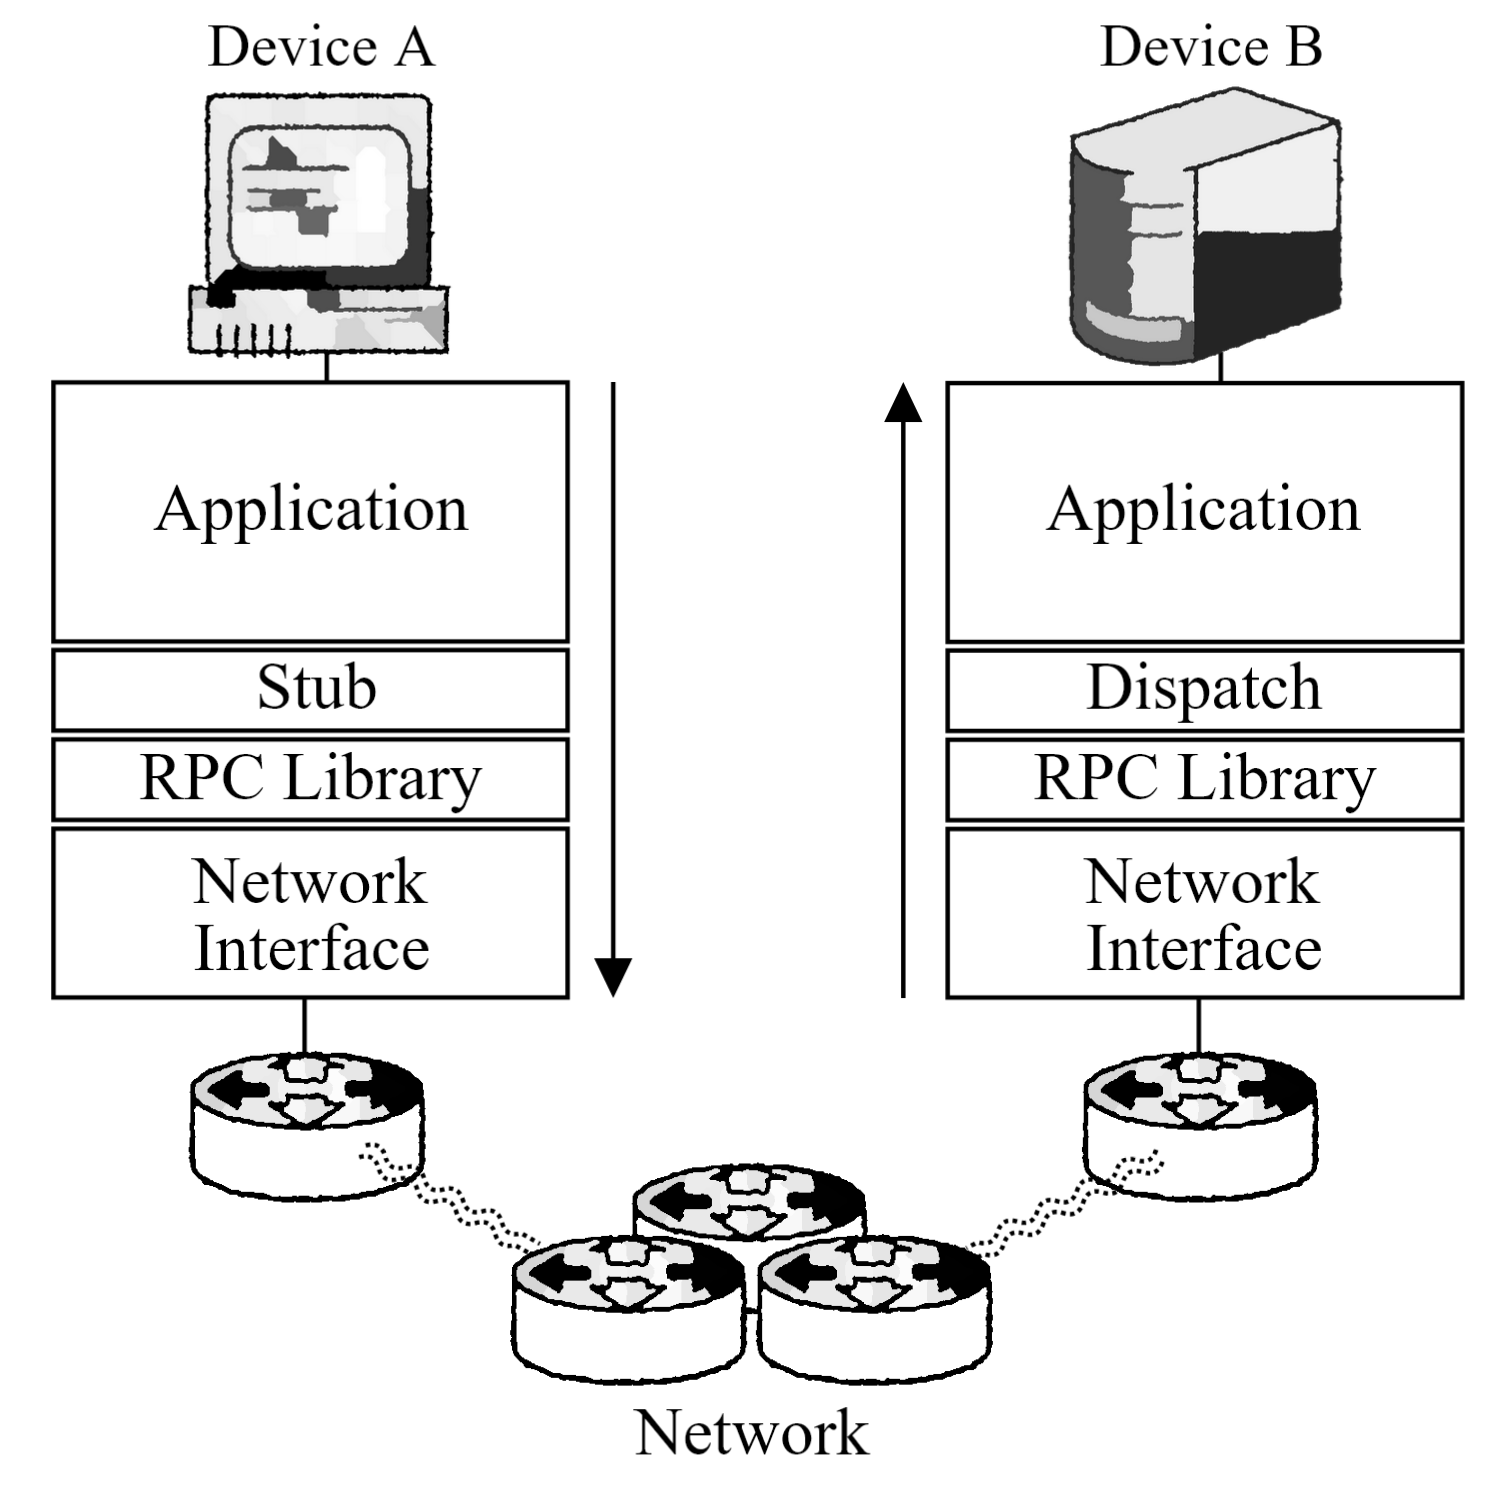
\includegraphics[width=0.55\textwidth]{Sections/rpc/rpc_stack.png}
    \caption{Client system $A$ making a request to Server system $B$ over RPC.}
    \label{fig:rpc_stack}
\end{figure}

\noindent
In terms of time it might look like:

\begin{figure}[h]
    \centering
    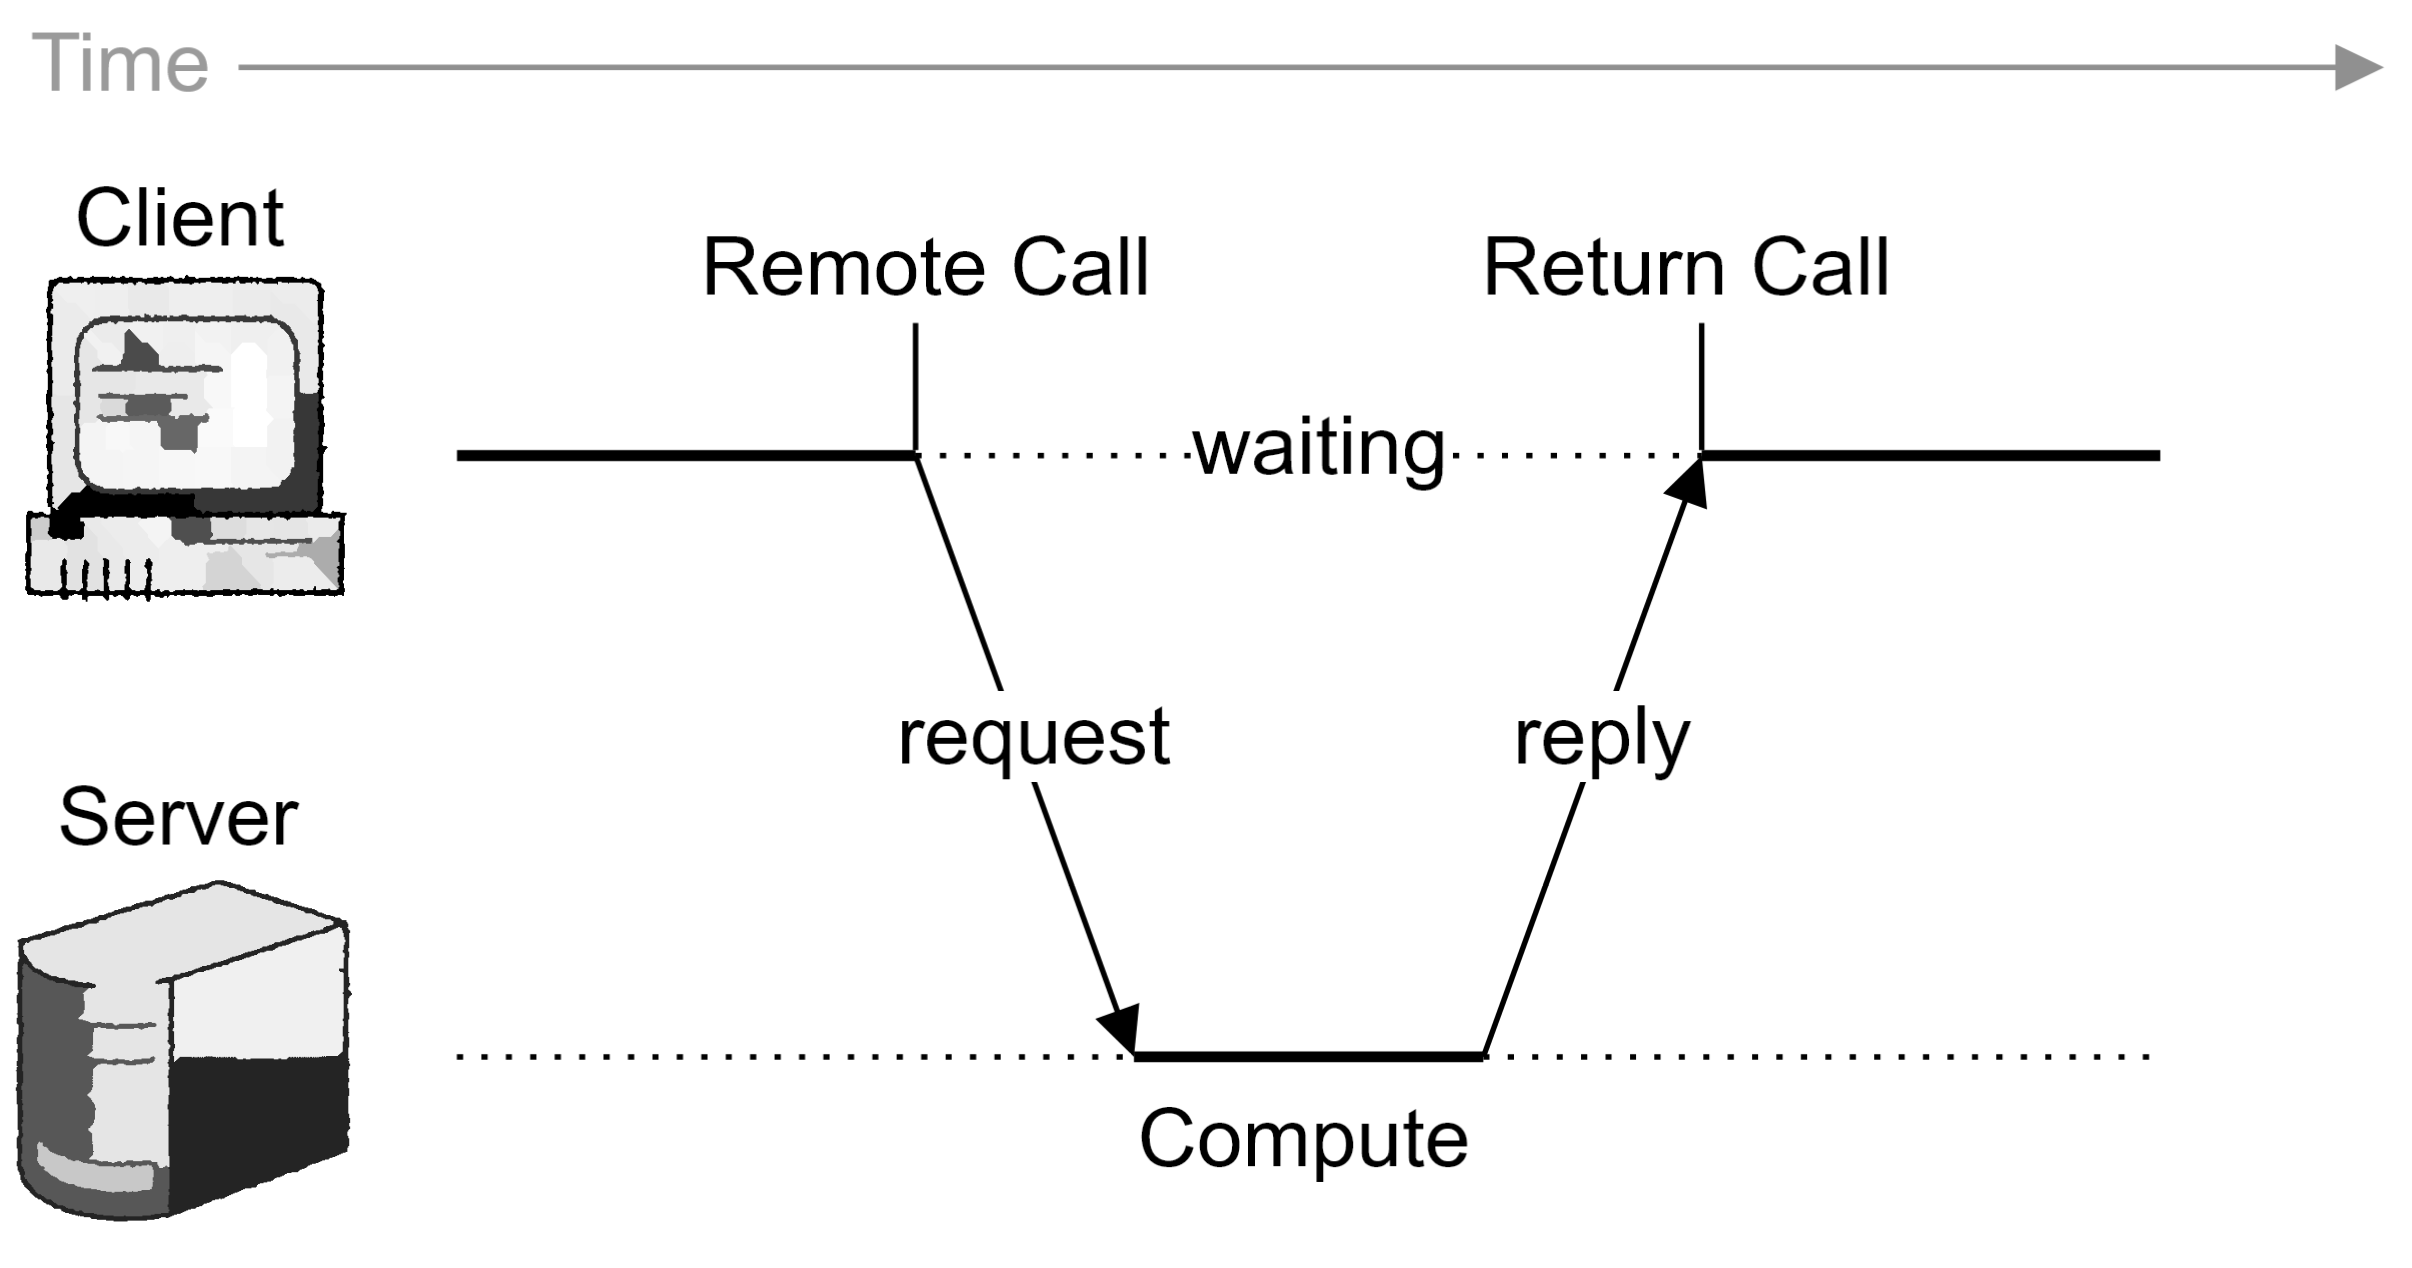
\includegraphics[width=0.6\textwidth]{Sections/rpc/call_time.png}
    \caption{RPC call stack over time.}
    \label{fig:rpc_time}
\end{figure}

\noindent 
Once the client makes the call it waits for the server to process the request and return the result. The programmer need not worry beyond sending the request and receiving the response.
The RPC deals with all the heavy work of facilitating the communication.

\newpage 

\noindent
Now to discuss what marshaling and unmarshaling are:
\begin{Def}[Marshaling and Unmarshaling]

    \textbf{Marshaling} handles data format conversions, converting the object into a byte stream (binary data).
    This conversion is known as \textbf{serialization}. This is done as the network can only transmit bytes\\
    
    \noindent
    \textbf{Unmarshaling} is the process of converting the byte stream into the original object called \textbf{deserialization}. 
    This allows the server to process the request.
\end{Def}

\noindent
To illustrate serialization and deserialization, consider the following diagram:
\begin{figure}[h]
    \centering
    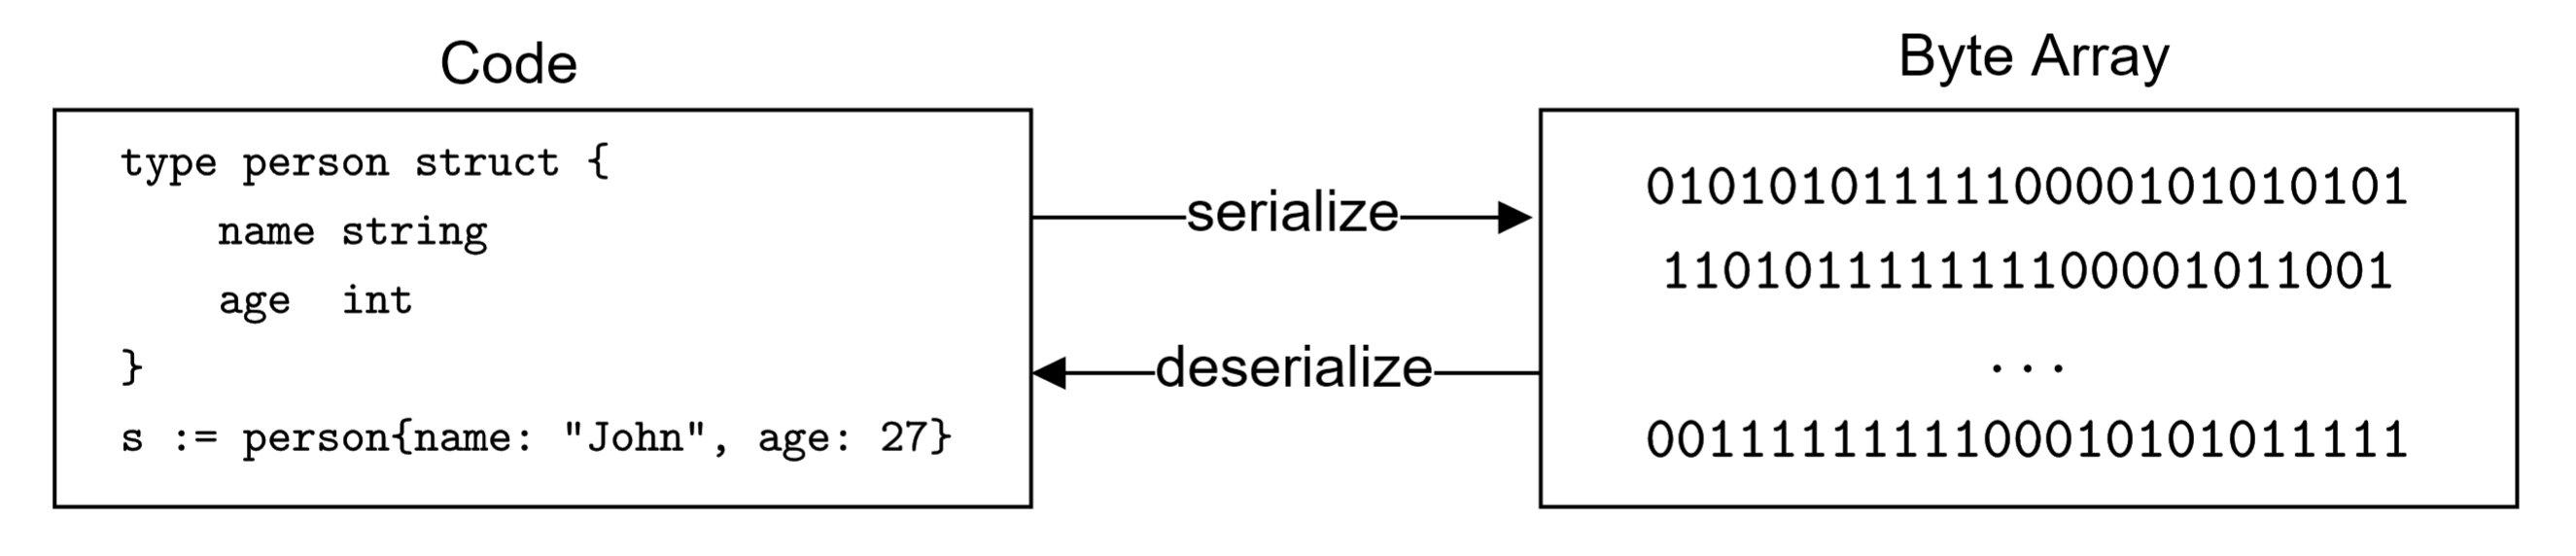
\includegraphics[width=1\textwidth]{Sections/rpc/ser.png}
    \caption{Serialization and Deserialization of data.}
    \label{fig:ser_deser}
\end{figure}

\noindent
There is one cardinal rule to remember when dealing with RPCs:
\begin{theo}[Network Reliability]

    \begin{center}
        \Large{\textbf{The network is always unreliable.}}
    \end{center}

    \vspace{1em}

    \noindent
    That is to say, the network can drop packets, delay messages, or deliver them out of order. Anything that 
    can go wrong will go wrong.
\end{theo}

\noindent
To handle network unreliability, we'll first consider two failure models:

\begin{Def}[At-least-once \& At-most-once]

    \begin{itemize}
        \item \textbf{At-least-once:} Regardless of failures, make the RPC call until the server responds. Works for read-only operations, otherwise, a strategy to handle duplicate requests is needed.
        \item \textbf{At-most-once:} Ensure the RPC call is made only once, even if the server fails to respond. This is done by having a unique identifier for each request. Each subsequent request 
        tells the server which calls have already been processed.
    \end{itemize}
\end{Def}

\newpage

\noindent
For our communication to work \textit{reliably} we need At-least-once and At-most-once with unlimited tries coupled by 
a fault-tolerant implementation. This brings us to the \textbf{GO RGC library}.

\begin{Def}[Go RPC Library]

    The Go RPC library provides a simple way to implement RPCs in the programming language Go. This gives us:
    \begin{itemize}
        \item At-most-once model with respect to a single
        client-server
        \item Built on top of single \textbf{TCP connection} (Transport Layer Protocol). This protocol ensures reliable communication between client and server.
        \item Returns error if reply is not received, e.g.,
        connection broken (TCP timeout)
    \end{itemize}
\end{Def}

\noindent
Now to discuss briefly how a basic TCP connection is made:
\begin{Def}[Establishing a TCP Connection (SYN ACK)]

    First a three-way handshake is a method used in a TCP/IP network to create a connection between a local host/client and server. 
    It is a three-step method that requires both the client and server to exchange \textbf{SYN (synchronize)}
     and \textbf{ACK (acknowledgment)}.
     \begin{enumerate}
        \item The client sends a SYN packet to the server requesting to synchronize sequence numbers.
        \item The server responds with a SYN-ACK packet, acknowledging the request and sending its own SYN request.
        \item The client responds with an ACK packet, acknowledging the server's SYN request.
     \end{enumerate}
    
    \noindent
    After the three-way handshake, the connection is established and the client and server can communicate exchanging SYN and ACK data-packets.
    To end the connection another three-way handshake takes placed, where instead of SYN, \textbf{FIN (finish)} is used.
    
\end{Def}

\noindent
Given this implementation, we approach somewhere in the realm of an \textbf{Exactly-Once model}:

\begin{Def}[Exactly-Once Model]

    The Exactly-Once model guarantees that a message is delivered exactly once to the recipient. Meaning, messages aren't duplicated, lost, or delivered out of order.
    However, In practice, data packets might do all of the above. Though with the right
    protocols in place, we can ensure order of logic is preserved.
\end{Def}

\newpage 
\noindent
Below we illustrate a simple TCP connection:
\begin{figure}[h]
    \centering
    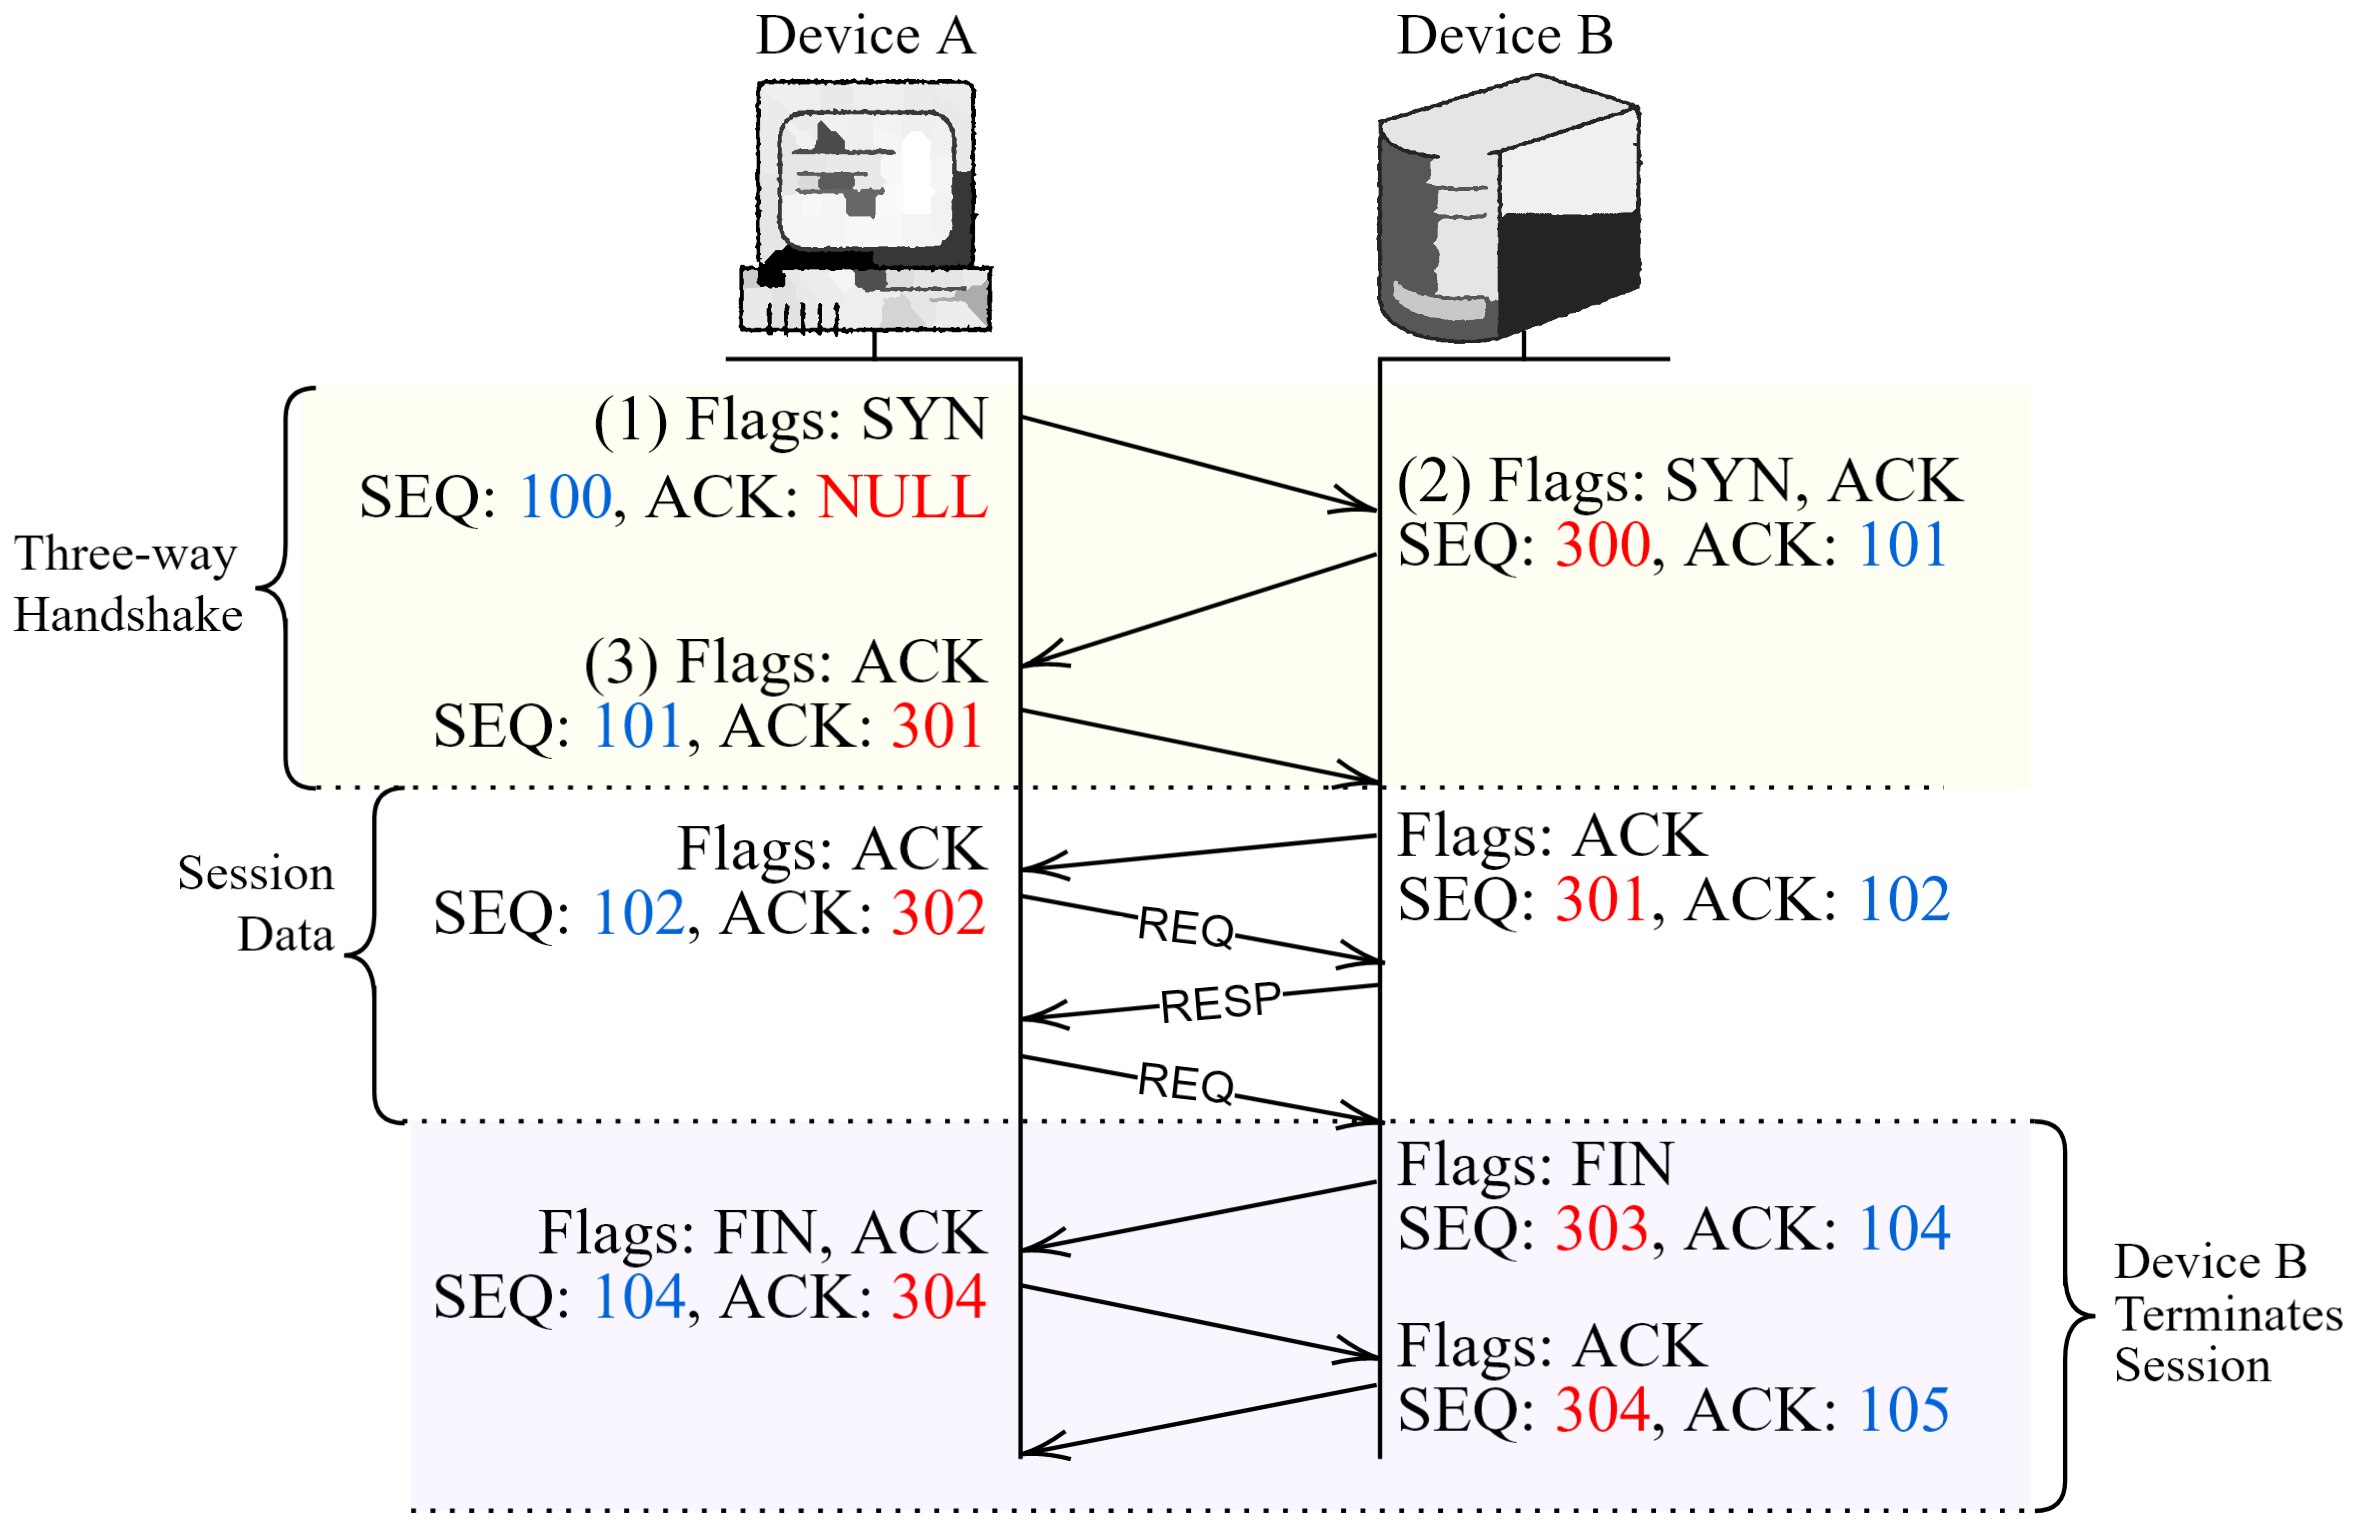
\includegraphics[width=.9\textwidth]{Sections/rpc/sync.png}
    \caption{TCP Handshake, data transfer, and session termination.}
    \label{fig:tcp}
\end{figure}

\noindent
Here the client (Device A) begins a three-way handshake with the server (Device B) to establish a connection. Both start with 
arbitrary sequence numbers for security purposes. With each packet received the two devices increment their sequence numbers accordingly.\\

\begin{Tip} If there still resides curiosity for the networking aspect of RPCs, consider reading our other notes:
    \href{https://github.com/Concise-Works/Cyber-Security/blob/main/main.pdf}{https://github.com/Concise-Works/Cyber-Security/blob/main/main.pdf}
\end{Tip}